% 实验报告模板

% 导言区
\documentclass[a4paper]{article}
\usepackage{report-style}
% 定义封面样式

% 单人报告封面样式
\def\singlecover
{
    \begin{titlepage}
        \centering
        \vspace{1cm}
        % 插入图片并调整文件名和路径
        
\includegraphics[width=0.5\textwidth]{./logo.jpg}
        \par\vspace{1cm}
        % 标题
        {\Huge \heiti \bf 课程名称 \par}
        \vspace{0.5cm}
        {\LARGE \heiti \bf 实验标题 \par}
        \vspace{1cm}
        % 作者
        \begin{center}
            \vspace{0.5cm}
            姓名\quad 学号\quad 班级\\
        \end{center}
        % 日期
        \vspace{0.5cm}
        {日期}
    \end{titlepage}
}

% 小组报告封面样式
\def\groupcover
{
    \begin{titlepage}
        \centering
        \vspace{1cm}
        % 插入图片并调整文件名和路径
        
\includegraphics[width=0.5\textwidth]{./logo.jpg}
        \par\vspace{1cm}
        % 标题
        {\Huge \heiti \bf 课程名称 \par}
        \vspace{0.5cm}
        {\LARGE \heiti \bf 实验标题 \par}
        \vspace{1cm}
        % 组员信息
        \section*{成员}
        \begin{center}
            \vspace{0.5cm}
            成员1\quad 学号1\quad 班级1\\
            成员2\quad 学号2\quad 班级2\\
            成员3\quad 学号3\quad 班级3\\
        %其余组员信息类似地添加
        \end{center}
        %分工情况
        \vspace{0.5cm}
        \section*{分工情况}
        \begin{center}
            \begin{tabular}{l}
                成员1\quad 成员1负责内容 \\
                成员2\quad 成员2负责内容 \\
                成员3\quad 成员3负责内容 \\
            \end{tabular}
        \end{center}
        % 日期
        \vspace{0.5cm}
        {日期}
    \end{titlepage}
}

\begin{document}

% 生成单人报告封面
\singlecover
% 生成小组报告封面
\groupcover

% 前言

\pagenumbering{Roman} % 前言部分设置为罗马数字页码
\sectionfont{\centering} % 章节标题居中

% 摘要

\section*{摘要}
\addcontentsline{toc}{section}{摘要}

本实验报告模板基于\href{https://github.com/AlmostGPH}{高鹏鸿}学长的\href{https://github.com/AlmostGPH/SDU-Latex-Template-for-Document}{实验报告模板}实现,在GNU通用公共许可证下发布。

本模板按照我的个人喜好,采用较为简洁清爽的风格,去除了高鹏鸿学长的模板中关于页眉页脚的相关内容。此外,将实现代码块的宏包更改为 \mintinline{text}{minted} ,以实现对多种语言语法高亮的支持,但也同时带来一些使用上的不便,需要对编译器及环境做一定配置,具体内容在正文部分中有所介绍。

本实验报告模板的默认内容将介绍如何使用该 \LaTeX 实验报告模板来编写实验报告,包括了一些基本的使用方法,如插入图片、插入代码、插入表格、插入公式、插入参考文献、插入超链接、插入脚注、绘制图像等,和此模板专有的方法,如插入封面等,以及一些个性化相关的内容。

如果在使用本模板时遇到任何问题,或对本模板有任何改进建议,请通过 \href{edgeworthlau@outlook.com}{edgeworthlau@outlook.com} 联系我。

% 目录

\newpage
\addcontentsline{toc}{section}{目录}
\hypersetup{linkcolor=black} % 设置目录中的链接颜色为黑色
\tableofcontents
\hypersetup{linkcolor=blue} % 恢复目录以外的链接颜色
\newpage

% 正文

\pagenumbering{arabic} % 正文部分设置为阿拉伯数字页码
\sectionfont{} % 章节标题左对齐


\section{基本使用}

\subsection{段落与空行}

在代码中直接输入文字即可新建一个段落。段落默认有首行缩进,若需取消一个段落的首行缩进,可在段落文字前添加 \mintinline{latex}{\noindent}。

在文字间使用空行分隔不同段落,请注意该空行不会渲染输出至文档中。若需要在文档中的段落间添加空行,可在对应位置添加 \mintinline{latex}{\vspace{0.5cm}}。

下面以\cref{lst:1} 中的代码为例,展示段落与空行相关命令的使用方法。

\begin{center}
    \captionof{listing}{段落与空行示例代码}
    \label{lst:1}
    \begin{minted}{latex}
这是段落一,该段未作任何设置。

\noindent 这是段落二,该段取消了首行缩进。

\vspace{0.5cm}

这是段落三,该段与前一段之间添加了空行。
    \end{minted}
\end{center}

\cref{lst:1} 中的代码经过编译后,输出结果如下所示。(为了更好地区分示例内容,后续大部分示例代码的输出内容均用两条分割线包裹。)

\vspace{0.75cm}
\hrule
\vspace{0.25cm}

这是段落一,该段未作任何设置。

\noindent 这是段落二,该段取消了首行缩进。

\vspace{0.5cm}

这是段落三,该段与前一段之间添加了空行。

\vspace{0.25cm}
\hrule
\vspace{0.25cm}

\subsection{逐项输出环境}

使用 \mintinline{latex}{\begin{itemize}...\end{itemize}} 环境可实现逐项输出。在环境中,使用 \mintinline{latex}{\item} 命令标记项,\mintinline{latex}{\subitem} 命令标记子项,\mintinline{latex}{\subsubitem}  命令标记二级子项。

下面以\cref{lst:2} 中的代码为例,展示逐项输出环境的使用方法。

\begin{center}
    \captionof{listing}{逐项输出示例代码}
    \label{lst:2}
    \begin{minted}{latex}
\begin{itemize}
    \item 第一项
    \item 第二项
    \subitem 第二项子项
    \subsubitem 第二项二级子项
    \item 第三项
\end{itemize}
    \end{minted}
\end{center}

\cref{lst:2} 中的代码经过编译后,输出结果如下所示。

\vspace{0.75cm}
\hrule
\vspace{0.25cm}

\begin{itemize}
    \item 第一项
    \item 第二项
    \subitem 第二项子项
    \subsubitem 第二项二级子项
    \item 第三项
\end{itemize}

\vspace{0.25cm}
\hrule
\vspace{0.25cm}

\subsection{分栏}

使用 \mintinline{latex}{\begin{multicols}{n}...\end{multicols}} 环境可实现分栏输出,其中 \mintinline{latex}{n} 为分栏数。在环境中,使用 \mintinline{latex}{\columnbreak} 命令可手动切换至下一栏。

更多使用方式可以查看 \href{https://www.overleaf.com/learn/latex/Multiple_columns}{Overleaf 的文档}。

下面以\cref{lst:3} 中的代码为例,展示分栏环境的使用方法。

\begin{center}
    \captionof{listing}{分栏示例代码}
    \label{lst:3}
    \begin{minted}{latex}
\begin{multicols}{2} % 指定分栏数为2
    这是左栏

    hello world

    \columnbreak % 手动切换至下一栏

    这是右栏

    你好世界
\end{multicols}
    \end{minted}
\end{center}

\cref{lst:3} 中的代码经过编译后,输出结果如下所示。

\vspace{0.75cm}
\hrule
\vspace{0.25cm}

\begin{multicols}{2} % 指定分栏数为2
    这是左栏

    hello world

    \columnbreak % 手动切换至下一栏

    这是右栏

    你好
\end{multicols}

\vspace{0.25cm}
\hrule
\vspace{0.25cm}

\section{插入图片}

\subsection{插入图片}

使用 \mintinline{latex}{\includegraphics[options]{figname}} 命令可插入图片,其中 \mintinline{latex}{options} 为图片选项,\mintinline{latex}{figname} 为图片文件名。

使用 \mintinline{latex}{\begin{figure}[htbp]...\end{figure}} 环境可实现对图片的浮动设置,其中 \mintinline{latex}{htbp} 用于设置图片位置,\mintinline{latex}{h}表示here,\mintinline{latex}{t}表示top,\mintinline{latex}{b}表示bottom,\mintinline{latex}{p}表示page。

下面以\cref{lst:4} 中的代码为例,展示插入图片相关命令的使用方法。

\begin{center}
    \captionof{listing}{插入图片示例代码}
    \label{lst:4}
    \begin{minted}{latex}
\begin{figure}[htbp]
    \begin{center}
        
\includegraphics[width=0.8\textwidth]{logo.jpg}
        % width调整图片大小
        \caption{Logo of SDU}
        \label{fig:1}
    \end{center}
\end{figure}
    \end{minted}
\end{center}

\cref{lst:4} 中的代码经过编译后,输出结果如\cref{fig:1} 所示。

\subsection{标题与标签}

使用 \mintinline{latex}{\caption{title}} 命令可添加标题,其中 \mintinline{latex}{title} 为标题内容。

使用 \mintinline{latex}{\captionof{type}{title}} 命令可为已知类型的内容添加标题,其中 \mintinline{latex}{type} 为类型,\mintinline{latex}{title} 为标题内容,最终生成的标题会包含:类型前缀、编号以及标题内容。

使用 \mintinline{latex}{\label{key}} 命令可添加标签,其中 \mintinline{latex}{key} 为标签名。

上述命令在插入其他内容时也常使用。

\begin{figure}[htbp]
    \begin{center}
        
\includegraphics[width=0.5\textwidth]{logo.jpg}
        % width调整图片大小
        \caption{Logo of SDU}
        \label{fig:1}
    \end{center}
\end{figure}

\begin{figure}[htbp]
    \centering
    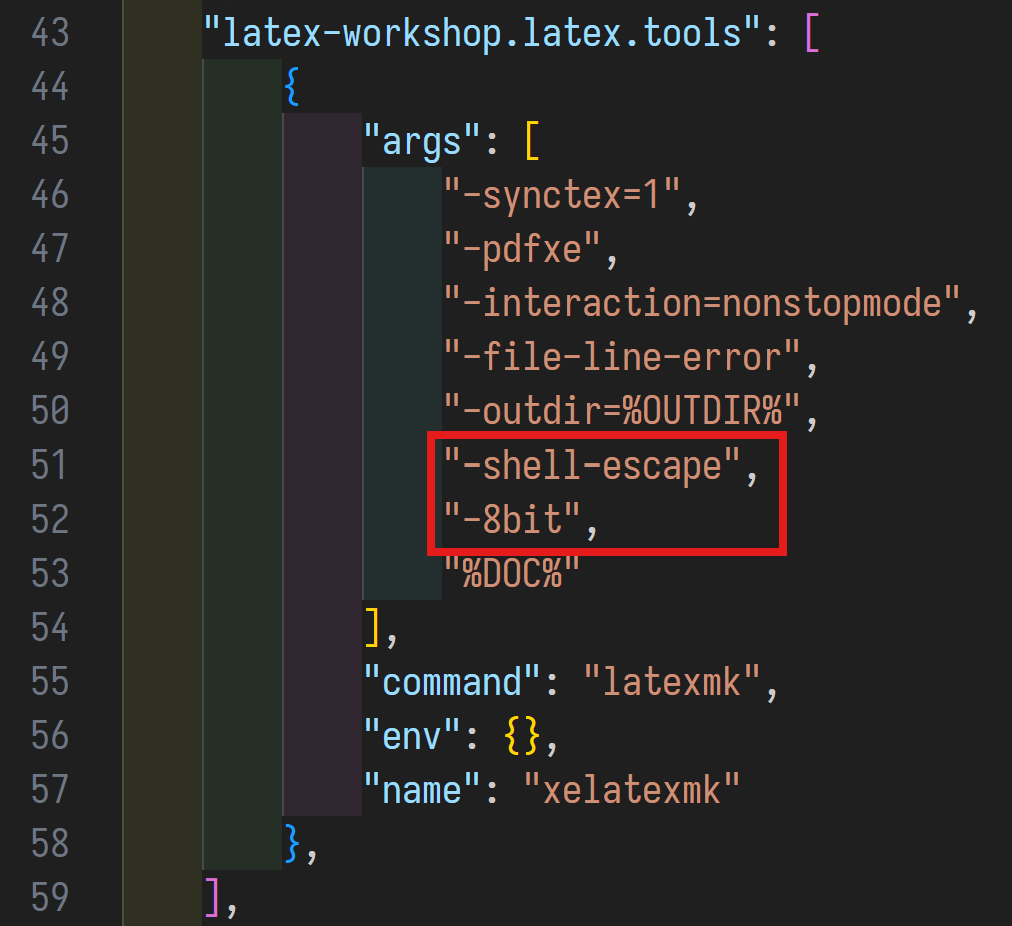
\includegraphics[width=0.8\textwidth]{imgs/vscode_setting.png}
    \caption{vscode 配置示例}
    \label{fig:2}
\end{figure}

\section{插入代码}

本模板使用 \mintinline{text}{minted} 宏包来实现对多种语言语法高亮的支持。由于 \mintinline{text}{minted} 宏包依赖于Python的 \mintinline{text}{Pygments} 包,且需要在编译时指定 \mintinline{bash}{-shell-escape} 选项,故需要对编译器及环境做一定配置。

下面的配置以 vscode 为例,其他编辑器类似。

打开 vscode 后,按下 \mintinline{text}{Ctrl + Shift + P},在命令面板中输入 \mintinline{text}{settings},选择 \mintinline{text}{Preferences: Open User Settings (JSON)},在打开的 \mintinline{text}{settings.json} 文件中找到 latex-workshop.latex.tools 选项,在所使用的编译器的参数中添加 \mintinline{bash}{-shell-escape} 和 \mintinline{bash}{-8bit} 两项,如\cref{fig:2} 所示。

其中,\mintinline{bash}{-shell-escape} 选项用于允许编译器调用 \mintinline{text}{Pygments} 环境; \mintinline{bash}{-8bit} 选项用于解决 \mintinline{text}{minted} 宏包在中文环境下的编码问题,以避免在缩进处渲染奇怪的符号。

此外,在使用 \mintinline{text}{minted} 宏包前,还需在环境中安装 \mintinline{text}{Pygments} 环境。使用 \mintinline{text}{pip} 或使用系统包管理器可完成安装,具体的安装步骤依不同的系统环境及版本可能有所变化,请搜索互联网以获得最新、最准确的安装步骤。

下面仅展示 \mintinline{text}{minted} 宏包的简单使用方法,更多使用方式可以查看 \href{https://mirror.math.princeton.edu/pub/CTAN/macros/latex/contrib/minted/minted.pdf}{\mintinline{text}{minted} 宏包的官方文档}。

\subsection{插入行内代码}

使用 \mintinline{latex}{\mintinline{language}{code}} 命令可插入行内代码,其中 \mintinline{latex}{language} 为代码语言,\mintinline{latex}{code} 为代码内容。

下面以\cref{lst:5} 中的代码为例,展示插入行内代码相关命令的使用方法。

\begin{center}
    \captionof{listing}{插入行内代码示例代码}
    \label{lst:5}
    \begin{minted}{latex}
这是一个插入了行内代码的示例段落,其中包含了 \mint{python}{print("Hello, world!")} 这行代码。
    \end{minted}
\end{center}

\cref{lst:5} 中的代码经过编译后,输出结果如下所示。

\vspace{0.75cm}
\hrule
\vspace{0.25cm}

这是一个插入了行内代码的示例段落,其中包含了 \mintinline{python}{print("Hello, world!")} 这行代码。

\vspace{0.25cm}
\hrule
\vspace{0.25cm}

\subsection{插入行间代码}

使用 \mintinline{latex}{\begin{minted}{language}...\end{minted}} 环境可插入行间代码,其中 \mintinline{latex}{language} 为代码语言。

使用 \mintinline{latex}{\inputminted{language}{filename}} 命令可插入外部代码文件,其中 \mintinline{latex}{language} 为代码语言,\mintinline{latex}{filename} 为代码文件名。

下面以\cref{lst:6} 中的代码为例,展示插入行间代码相关命令的使用方法。

\begin{center}
    \captionof{listing}{插入行间代码示例代码}
    \label{lst:6}
    \inputminted{latex}{codes/example.tex}
\end{center}

请注意,在使用 \mintinline{text}{minted} 展示 \LaTeX 代码时,代码中的 \mintinline{latex}{\end{minted}} 会使编译器无法分辨代码的结束位置,导致编译失败。为解决此问题,可将待展示的\LaTeX 代码写入一个文件中,以插入外部代码文件展示。

\cref{lst:6} 中的代码经过编译后,输出结果如\cref{lst:7} 所示。

\begin{center}
    \captionof{listing}{插入行间代码输出结果}
    \label{lst:7}
    \begin{minted}{python}
def extended_gcd(a, b):
    if b == 0:
        return (a, 1, 0)
    else:
        d, x, y = extended_gcd(b, a % b)
        return (d, y, x - (a // b) * y)

def mod_inverse(a, m):
    d, x, y = extended_gcd(a, m)
    if d != 1:
        raise ValueError("Modular inverse does not exist")
    else:
        return x % m
    \end{minted}
    \inputminted{python}{codes/example.py}
\end{center}

\section{插入表格}

使用 \mintinline{latex}{\begin{tabular}{set}... \end{tabular}} 环境可插入表格,其中 \mintinline{latex}{set} 为表示表格的列数和对齐方式的字符串,\mintinline{latex}{|} 表示在表格中添加单竖线,\mintinline{latex}{||} 表示在表格中添加双竖线,\mintinline{latex}{c} 表示居中对齐,\mintinline{latex}{l} 表示左对齐,\mintinline{latex}{r} 表示右对齐。在环境中,使用 \mintinline{latex}{\hline} 可添加横线,使用 \mintinline{latex}{&} 可分隔单元格,使用 \mintinline{latex}{\\} 可换行。

下面以\cref{lst:8} 中的代码为例,展示插入表格相关命令的使用方法。

\begin{center}
    \captionof{listing}{插入表格示例代码}
    \label{lst:8}
    \begin{minted}{latex}
\begin{center}
    \captionof{table}{表格示例1}
    \label{tab:tab1}
    \begin{tabular}{|c|c|c|}   
        \hline
        A & B & C \\
        \hline
        1 & 2 & 3 \\
        \hline
        4 & 5 & 6 \\
        \hline
        7 & 8 & 9 \\
        \hline
    \end{tabular}
\end{center}

\begin{center}
    \captionof{table}{表格示例2}
    \label{tab:2}
    \begin{tabular}{r||l c|}
        \hline
        AA & BB & C \\
        \hline
        1 & 2 & 3 \\
        4 & 5 & 6 \\
        \hline
        \hline
        7 & 8 & 9 \\
    \end{tabular}
\end{center}
    \end{minted}
\end{center}

\cref{lst:8} 中的代码经过编译后,输出结果如\cref{tab:1} 和 \cref{tab:2} 所示。

\begin{center}
    \captionof{table}{表格示例1}
    \label{tab:1}
    \begin{tabular}{|c|c|c|}   
        \hline
        A & B & C \\
        \hline
        1 & 2 & 3 \\
        \hline
        4 & 5 & 6 \\
        \hline
        7 & 8 & 9 \\
        \hline
    \end{tabular}
\end{center}

\begin{center}
    \captionof{table}{表格示例2}
    \label{tab:2}
    \begin{tabular}{r||l c|}
        \hline
        AA & BB & C \\
        \hline
        1 & 2 & 3 \\
        4 & 5 & 6 \\
        \hline
        \hline
        7 & 8 & 9 \\
    \end{tabular}
\end{center}

\section{插入公式}

如果不熟悉 \LaTeX 的公式语法,可以使用 \href{https://www.codecogs.com/latex/eqneditor.php}{CodeCogs} 来生成公式的代码。

\subsection{插入行内公式}

使用 \mintinline{latex}{$...$} 或 \mintinline{latex}{\(...\)} 插入行内公式。

下面以\cref{lst:9} 中的代码为例,展示插入行内公式相关命令的使用方法。

\begin{center}
    \captionof{listing}{插入行内公式示例代码}
    \label{lst:9}
    \begin{minted}{latex}
这是一个插入了行内公式的示例段落,其中包含了 $a^2 + b^2 = c^2$ 和  \((a+b)^2 = a^2 + 2ab + b^2\) 这两个公式。
    \end{minted}
\end{center}

\cref{lst:9} 中的代码经过编译后,输出结果如下所示。

\vspace{0.75cm}
\hrule
\vspace{0.25cm}

这是一个插入了行内公式的示例段落,其中包含了 $a^2 + b^2 = c^2$ 和  \((a+b)^2 = a^2 + 2ab + b^2\) 这两个公式。

\vspace{0.25cm}
\hrule
\vspace{0.25cm}

\subsection{插入行间公式}

使用 \mintinline{latex}{$$...$$} 或 \mintinline{latex}{\[...\]} 或 \mintinline{latex}{\begin{equation}...\end{equation}} 插入行间公式。

下面以\cref{lst:10} 中的代码为例,展示插入行间公式相关命令的使用方法。

\begin{center}
    \captionof{listing}{插入行间公式示例代码}
    \label{lst:10}
    \begin{minted}{latex}
这是一个插入了行间公式的示例段落,
$$
    \int_{0}^{1} x^2 \mathrm{d} x = \frac{1}{3}
$$
\[
    \int_{0}^{1} x^2 \mathrm{d} x = \frac{1}{3}
\]
\begin{equation}
    \int_{0}^{1} x^2 \mathrm{d} x = \frac{1}{3}
\end{equation}
在这个段落中,以三种不同的方式插入了相同的公式。
    \end{minted}
\end{center}

\cref{lst:10} 中的代码经过编译后,输出结果如下所示。

\vspace{0.75cm}
\hrule
\vspace{0.25cm}

这是一个插入了行间公式的示例段落,
$$
    \int_{0}^{1} x^2 \mathrm{d} x = \frac{1}{3}
$$
\[
    \int_{0}^{1} x^2 \mathrm{d} x = \frac{1}{3}
\]
\begin{equation}
    \int_{0}^{1} x^2 \mathrm{d} x = \frac{1}{3}
\end{equation}
在这个段落中,以三种不同的方式插入了相同的公式。

\vspace{0.25cm}
\hrule
\vspace{0.25cm}

\section{插入参考文献}

\subsection{插入内部参考文献}

使用 \mintinline{latex}{\label{key}} 定义标签,其中 \mintinline{latex}{key} 为标签名。

使用 \mintinline{latex}{\ref{key}} 引用标签,其中 \mintinline{latex}{key} 为带引用标签的标签名,使用时需手动添加标签类型前缀。

此外,本模板还使用 \mintinline{text}{cleveref} 宏包对引用命令进行了重定义,使用 \mintinline{latex}{\cref} 命令可实现对标签的引用,使用时无需再手动添加标签类型前缀。本模板已默认将“listing”“figure”“table”三个前缀重定义为“代码”“图”“表”,相关设置可以在 \mintinline{text}{report-style.sty} 文件中查看,可自行修改或增加其他类型前缀的重定义。

完成对标签的定义和引用后,在输出的文件中点击引用即可跳转至被引用位置。

下面以\cref{lst:11} 中的代码为例,展示插入内部参考文献相关命令的使用方法。

\begin{center}
    \captionof{listing}{插入内部参考文献示例代码}
    \label{lst:11}
    \begin{minted}{latex}
这是一个插入了内部参考文献的示例段落,其中包含了对图\ref{fig:1}和\cref{lst:7}的引用。
    \end{minted}
\end{center}

\cref{lst:11} 中的代码经过编译后,输出结果如下所示。

\vspace{0.75cm}
\hrule
\vspace{0.25cm}

这是一个插入了内部参考文献的示例段落,其中包含了对图\ref{fig:1}和\cref{lst:7}的引用。

\vspace{0.25cm}
\hrule
\vspace{0.25cm}

\subsection{插入外部参考文献}

使用 \mintinline{latex}{\begin{thebibliography}{set}...\end{thebibliography}} 环境定义外部参考文献,其中 \mintinline{latex}{set} 为设置参考文献编号方式,一般设置为 \mintinline{latex}{99},指定参考文献的项目按照数字进行编号且编号最大值为99。在环境中,使用 \mintinline{latex}{\bibitem{key}...} 定义参考文献,其中 \mintinline{latex}{key} 为参考文献的键,随后可添加文献的相关信息。一般来讲,应在附录部分定义参考文献。

使用 \mintinline{latex}{\cite{key}} 命令可插入外部参考文献,其中 \mintinline{latex}{key} 为参考文献的键。

下面以\cref{lst:12} 中的代码为例,展示插入外部参考文献相关命令的使用方法。

\begin{center}
    \captionof{listing}{插入外部参考文献示例代码}
    \label{lst:12}
    \begin{minted}{latex}
\begin{thebibliography}{99}
    \bibitem{1} 参考文献1
    \bibitem{2} 参考文献2
\end{thebibliography}

这是一个插入了外部参考文献的示例段落,其中包含了对参考文献1\cite{1}和参考文献2\cite{2}的引用。
    \end{minted}
\end{center}

\cref{lst:12} 中的代码经过编译后,输出结果如下所示。

\vspace{0.75cm}
\hrule
\vspace{0.25cm}

\begin{thebibliography}{99}
    \bibitem{1} 参考文献1
    \bibitem{2} 参考文献2
\end{thebibliography}

这是一个插入了外部参考文献的示例段落,其中包含了对参考文献1\cite{1}和参考文献2\cite{2}的引用。

\vspace{0.25cm}
\hrule
\vspace{0.25cm}

\section{插入超链接}

使用 \mintinline{latex}{\href{url}{text}} 命令可插入超链接,其中 \mintinline{latex}{url} 为链接地址,\mintinline{latex}{text} 为链接文本。

下面以\cref{lst:13} 中的代码为例,展示插入超链接相关命令的使用方法。

\begin{center}
    \captionof{listing}{插入超链接示例代码}
    \label{lst:13}
    \begin{minted}{latex}
\href{https://www.sdu.edu.cn/}{山东大学}是中国著名的综合性大学,位于山东省济南市。
    \end{minted}
\end{center}

\cref{lst:13} 中的代码经过编译后,输出结果如下所示。

\vspace{0.75cm}
\hrule
\vspace{0.25cm}

\href{https://www.sdu.edu.cn/}{山东大学}是中国著名的综合性大学,位于山东省济南市。

\vspace{0.25cm}
\hrule
\vspace{0.25cm}

\section{插入脚注}

使用 \mintinline{latex}{\footnote{text}} 命令可插入脚注,其中 \mintinline{latex}{text} 为脚注内容。

下面以\cref{lst:14} 中的代码为例,展示插入脚注相关命令的使用方法。

\begin{center}
    \captionof{listing}{插入脚注示例代码}
    \label{lst:14}
    \begin{minted}{latex}
这是一个插入了脚注的示例段落,其中包含了脚注\footnote{这是一个脚注},本页的末尾位置将展示脚注的具体内容。
    \end{minted}
\end{center}

\cref{lst:14} 中的代码经过编译后,输出结果如下所示。

\vspace{0.75cm}
\hrule
\vspace{0.25cm}

这是一个插入了脚注的示例段落,其中包含了脚注\footnote{这是一个脚注},本页的末尾位置将展示脚注的具体内容。

\vspace{0.25cm}
\hrule
\vspace{0.25cm}

\section{图表绘制}

使用 \mintinline{latex}{TikZ} 包可以绘制各种图像,例如流程图、树图等。

下面仅做简单的示例,详细的使用方式可以查看 \href{https://cn.overleaf.com/learn/latex/TikZ_package}{Overleaf的文档}。

\subsection{绘制流程图}

下面以\cref{lst:15} 中的代码为例,展示绘制流程图的方法。

\begin{center}
    \captionof{listing}{绘制流程图示例代码}
    \label{lst:15}
    \begin{minted}{latex}
\begin{figure}[htbp]
    \centering
    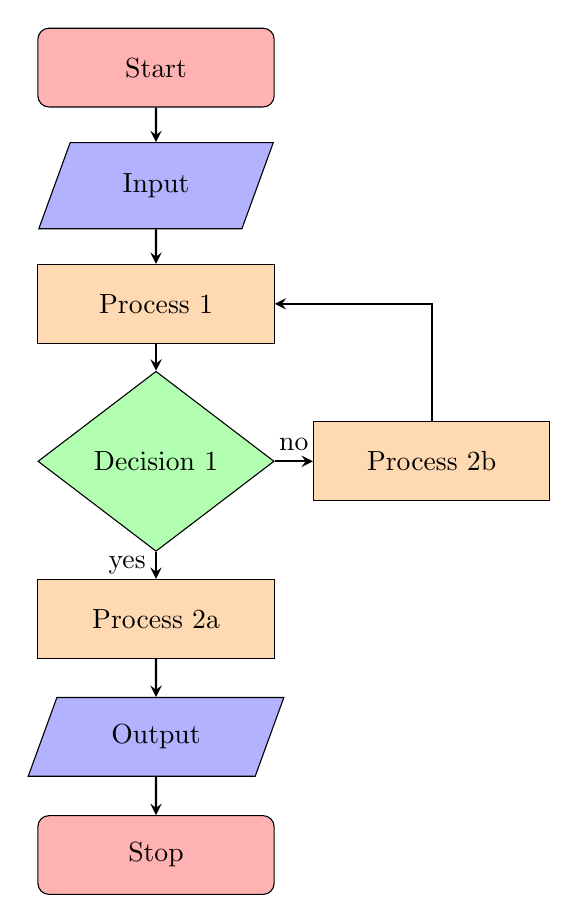
\begin{tikzpicture}[node distance=1.5cm]
        \usetikzlibrary{shapes,arrows}

        \tikzstyle{startstop} = [rectangle, rounded corners, minimum width=3cm, minimum height=1cm, text centered, draw=black, fill=red!30]
        \tikzstyle{io} = [trapezium, trapezium left angle=70, trapezium right angle=110, minimum width=3cm, minimum height=1cm, text centered, draw=black, fill=blue!30]
        \tikzstyle{process} = [rectangle, minimum width=3cm, minimum height=1cm, text centered, draw=black, fill=orange!30]
        \tikzstyle{decision} = [diamond, minimum width=3cm, minimum height=1cm, text centered, draw=black, fill=green!30]
        \tikzstyle{arrow} = [thick,->,>=stealth]

        \node (start) [startstop] {Start};
        \node (in1) [io, below of=start] {Input};
        \node (pro1) [process, below of=in1] {Process 1};
        \node (dec1) [decision, below of=pro1, yshift=-0.5cm] {Decision 1};
        \node (pro2a) [process, below of=dec1, yshift=-0.5cm] {Process 2a};
        \node (pro2b) [process, right of=dec1, xshift=2cm] {Process 2b};
        \node (out1) [io, below of=pro2a] {Output};
        \node (stop) [startstop, below of=out1] {Stop};
        
        \draw [arrow] (start) -- (in1);
        \draw [arrow] (in1) -- (pro1);
        \draw [arrow] (pro1) -- (dec1);
        \draw [arrow] (dec1) -- node[anchor=east] {yes} (pro2a);
        \draw [arrow] (dec1) -- node[anchor=south] {no} (pro2b);
        \draw [arrow] (pro2b) |- (pro1);
        \draw [arrow] (pro2a) -- (out1);
        \draw [arrow] (out1) -- (stop);
    \end{tikzpicture}
    \caption{流程图}
    \label{fig:flowchart}
\end{figure}
    \end{minted}
\end{center}

\cref{lst:15} 中的代码经过编译后,输出结果如\cref{fig:flowchart} 所示。

\vspace{0.75cm}

\begin{figure}[htbp]
    \centering
    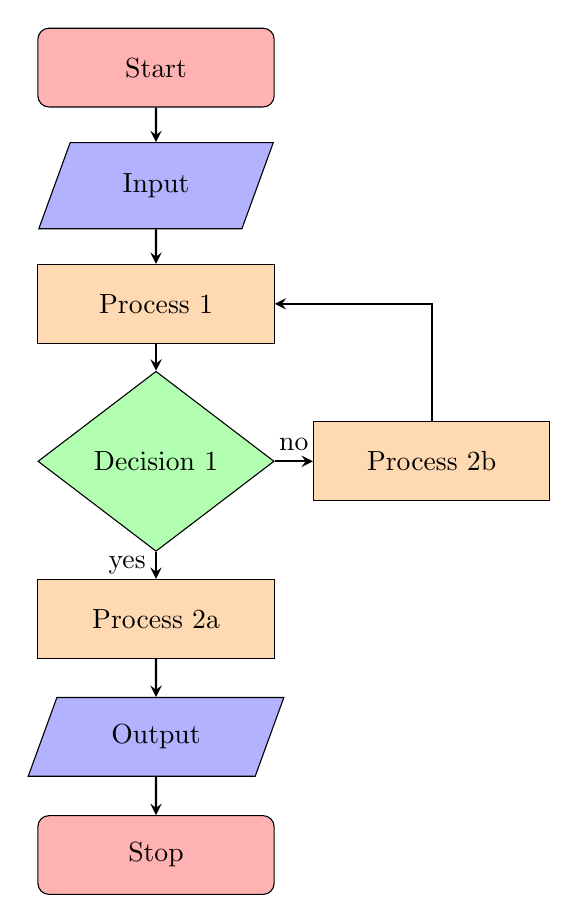
\begin{tikzpicture}[node distance=1.5cm]
        \usetikzlibrary{shapes,arrows}

        \tikzstyle{startstop} = [rectangle, rounded corners, minimum width=3cm, minimum height=1cm, text centered, draw=black, fill=red!30]
        \tikzstyle{io} = [trapezium, trapezium left angle=70, trapezium right angle=110, minimum width=3cm, minimum height=1cm, text centered, draw=black, fill=blue!30]
        \tikzstyle{process} = [rectangle, minimum width=3cm, minimum height=1cm, text centered, draw=black, fill=orange!30]
        \tikzstyle{decision} = [diamond, minimum width=3cm, minimum height=1cm, text centered, draw=black, fill=green!30]
        \tikzstyle{arrow} = [thick,->,>=stealth]

        \node (start) [startstop] {Start};
        \node (in1) [io, below of=start] {Input};
        \node (pro1) [process, below of=in1] {Process 1};
        \node (dec1) [decision, below of=pro1, yshift=-0.5cm] {Decision 1};
        \node (pro2a) [process, below of=dec1, yshift=-0.5cm] {Process 2a};
        \node (pro2b) [process, right of=dec1, xshift=2cm] {Process 2b};
        \node (out1) [io, below of=pro2a] {Output};
        \node (stop) [startstop, below of=out1] {Stop};
        
        \draw [arrow] (start) -- (in1);
        \draw [arrow] (in1) -- (pro1);
        \draw [arrow] (pro1) -- (dec1);
        \draw [arrow] (dec1) -- node[anchor=east] {yes} (pro2a);
        \draw [arrow] (dec1) -- node[anchor=south] {no} (pro2b);
        \draw [arrow] (pro2b) |- (pro1);
        \draw [arrow] (pro2a) -- (out1);
        \draw [arrow] (out1) -- (stop);
    \end{tikzpicture}
    \caption{流程图}
    \label{fig:flowchart}
\end{figure}

\subsection{绘制树图}

下面以\cref{lst:16} 中的代码为例,展示绘制树图的方法。

\begin{center}
    \captionof{listing}{绘制树图示例代码}
    \label{lst:16}
    \begin{minted}{latex}
\begin{figure}[htbp]
    \centering
    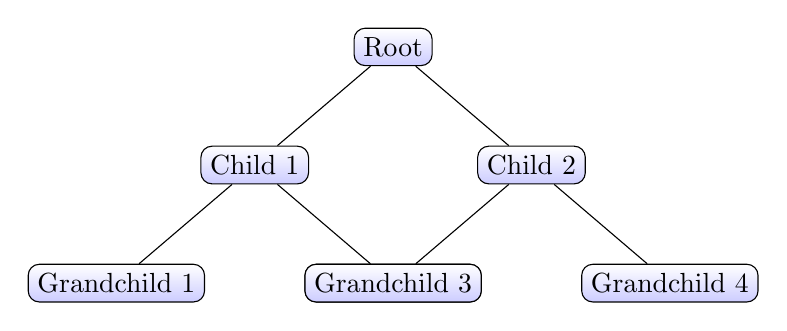
\begin{tikzpicture}[sibling distance=10em,
        every node/.style = {shape=rectangle,
            rounded corners, draw, align=center,
            top color=white, bottom color=blue!20}]
        \node {Root}
        child { node {Child 1} 
            child { node {Grandchild 1} }
            child { node {Grandchild 2} }
        }
        child { node {Child 2} 
            child { node {Grandchild 3} }
            child { node {Grandchild 4} }
        };
    \end{tikzpicture}
    \caption{树图}
    \label{fig:tree}
\end{figure}
    \end{minted}
\end{center}

\cref{lst:16} 中的代码经过编译后,输出结果如\cref{fig:tree} 所示。

\vspace{0.75cm}

\begin{figure}[htbp]
    \centering
    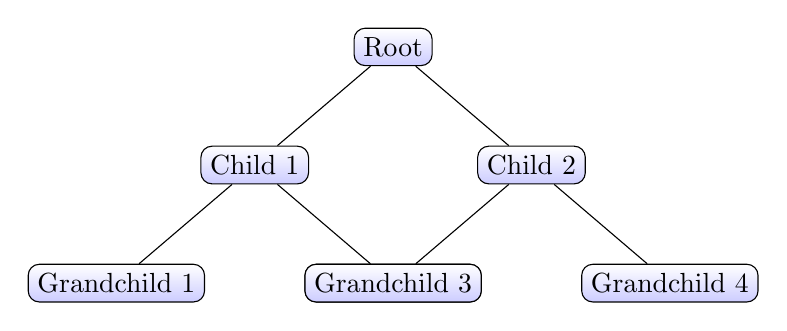
\begin{tikzpicture}[sibling distance=10em,
        every node/.style = {shape=rectangle,
            rounded corners, draw, align=center,
            top color=white, bottom color=blue!20}]
        \node {Root}
        child { node {Child 1} 
            child { node {Grandchild 1} }
            child { node {Grandchild 2} }
        }
        child { node {Child 2} 
            child { node {Grandchild 3} }
            child { node {Grandchild 4} }
        };
    \end{tikzpicture}
    \caption{树图}
    \label{fig:tree}
\end{figure}

\subsection{绘制拓扑图}

下面以\cref{lst:17} 中的代码为例,展示绘制拓扑图的方法。

\begin{center}
    \captionof{listing}{绘制拓扑图示例代码}
    \label{lst:17}
    \begin{minted}{latex}
\begin{figure}[htbp]
    \centering
    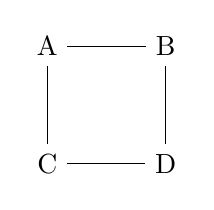
\begin{tikzpicture}
        \usetikzlibrary{positioning}

        \node (A) {A};
        \node (B) [right=of A] {B};
        \node (C) [below=of A] {C};
        \node (D) [below=of B] {D};

        \draw (A) -- (B);
        \draw (A) -- (C);
        \draw (B) -- (D);
        \draw (C) -- (D);
    \end{tikzpicture}
    \caption{拓扑图}
    \label{fig:topology}
\end{figure}
    \end{minted}
\end{center}

\cref{lst:17} 中的代码经过编译后,输出结果如\cref{fig:topology} 所示。

\vspace{0.75cm}

\begin{figure}[htbp]
    \centering
    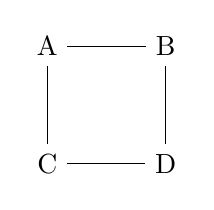
\begin{tikzpicture}
        \usetikzlibrary{positioning}

        \node (A) {A};
        \node (B) [right=of A] {B};
        \node (C) [below=of A] {C};
        \node (D) [below=of B] {D};

        \draw (A) -- (B);
        \draw (A) -- (C);
        \draw (B) -- (D);
        \draw (C) -- (D);
    \end{tikzpicture}
    \caption{拓扑图}
    \label{fig:topology}
\end{figure}

\subsection{绘制时序图}

下面以\cref{lst:18} 中的代码为例,展示绘制时序图的方法。

\begin{center}
    \captionof{listing}{绘制时序图示例代码}
    \label{lst:18}
    \begin{minted}{latex}
\begin{figure}[htbp]
    \centering
    \begin{tikzpicture}
        \draw (0,0) -- (0,1) -- (1,1) -- (1,0) -- (2,0) -- (2,1) -- (3,1) -- (3,0) -- (4,0);
    \end{tikzpicture}
    \caption{时序图}
    \label{fig:timing}
\end{figure}
    \end{minted}
\end{center}

\cref{lst:18} 中的代码经过编译后,输出结果如\cref{fig:timing} 所示。

\vspace{0.75cm}

\begin{figure}[htbp]
    \centering
    \begin{tikzpicture}
        \draw (0,0) -- (0,1) -- (1,1) -- (1,0) -- (2,0) -- (2,1) -- (3,1) -- (3,0) -- (4,0);
    \end{tikzpicture}
    \caption{时序图}
    \label{fig:timing}
\end{figure}

\subsection{绘制其他图形}

下面以\cref{lst:19} 中的代码为例,展示绘制其他图形的方法。

\begin{center}
    \captionof{listing}{绘制其他图形示例代码}
    \label{lst:19}
    \begin{minted}{latex}
\begin{figure}[htbp]
    \centering
    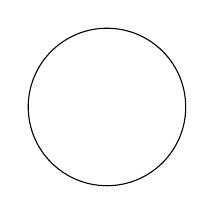
\begin{tikzpicture}
        \draw (0,0) circle [radius=1];
    \end{tikzpicture}
    \caption{其他图形}
    \label{fig:other}
\end{figure}
    \end{minted}
\end{center}

\cref{lst:19} 中的代码经过编译后,输出结果如\cref{fig:other} 所示。

\vspace{0.75cm}

\begin{figure}[htbp]
    \centering
    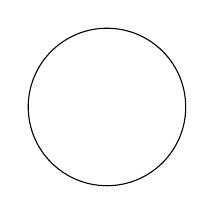
\begin{tikzpicture}
        \draw (0,0) circle [radius=1];
    \end{tikzpicture}
    \caption{其他图形}
    \label{fig:other}
\end{figure}

\subsection{使用Python绘图}

使用Python的 \mintinline{python}{matplotlib} 包绘图,将绘制结果输出为pdf文件,此时绘制的图表保存为矢量图,从而保证了图表的清晰度。随后,在需要使用图表时,按照插入图片的方式插入pdf文件即可。

\cref{lst:20} 展示了使用Python的 \mintinline{python}{matplotlib} 包绘制图表的示例代码。

\begin{center}
    \captionof{listing}{使用Python绘图示例代码}
    \label{lst:20}
    \inputminted{python}{codes/matplotlib.py}
\end{center}

下面以\cref{lst:21} 中的代码为例,展示插入Python绘制的图表的方法。

\begin{center}
    \captionof{listing}{插入Python绘制的图表示例代码}
    \label{lst:21}
    \begin{minted}{latex}
\begin{figure}[htbp]
    \begin{center}
        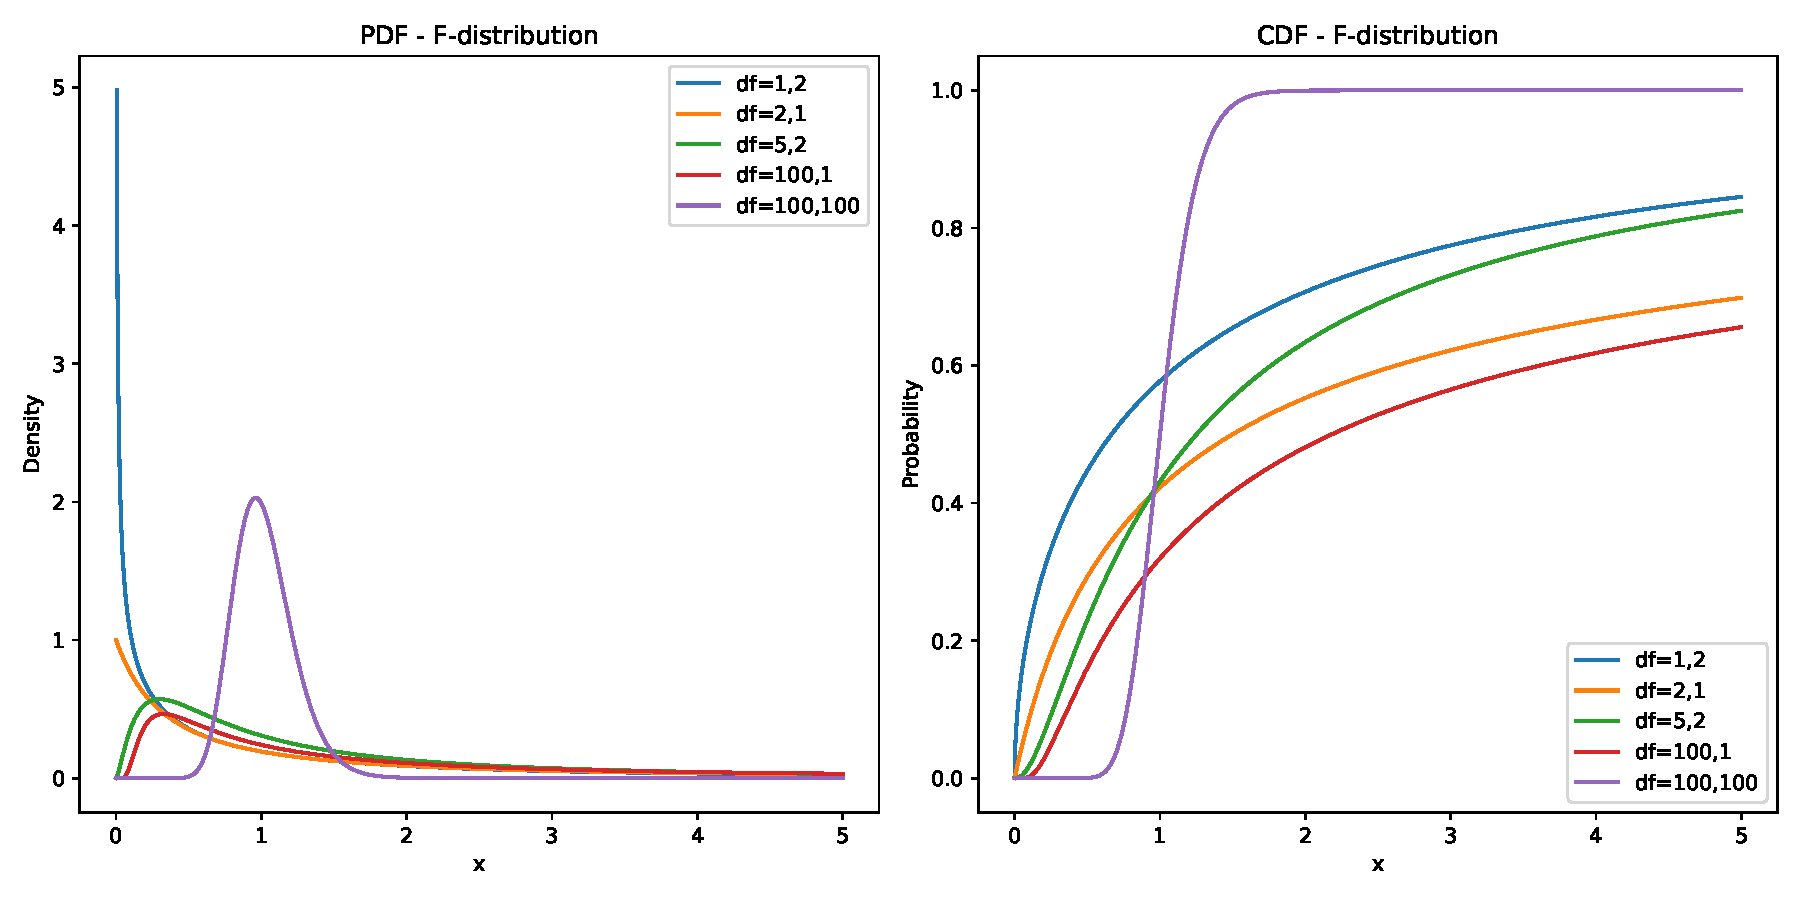
\includegraphics[width=0.8\textwidth]{imgs/plots.pdf}
        \caption{F分布}
        \label{fig:F}
    \end{center}
\end{figure}
    \end{minted}
\end{center}

\cref{lst:21} 中的代码经过编译后,输出结果如\cref{fig:F} 所示。

\vspace{0.75cm}

\begin{figure}[htbp]
    \begin{center}
        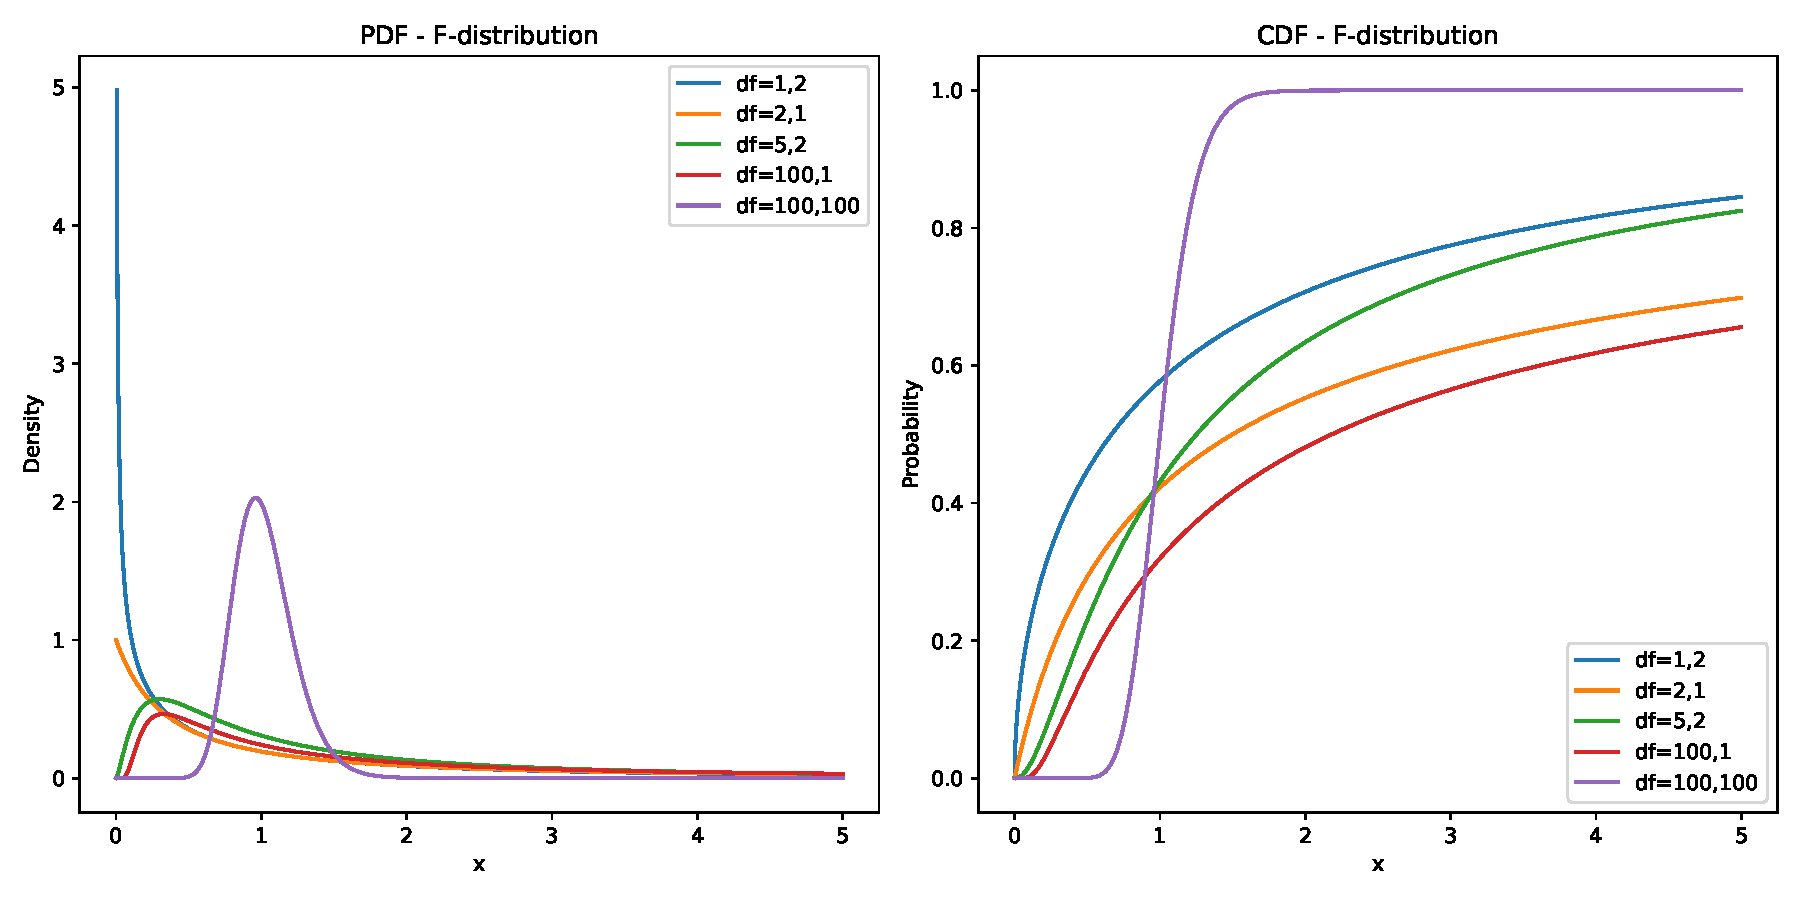
\includegraphics[width=\textwidth]{imgs/plots.pdf}
        \caption{F分布}
        \label{fig:F}
    \end{center}
\end{figure}

\section{插入封面}

本模板提供了两种封面样式,分别为“单人报告封面”和“小组报告封面”。其中,“单人报告封面”包含了课程名称、实验名称、姓名、学号、班级、提交日期等信息;“小组报告封面”包含了课程名称、实验名称、组员信息(姓名、学号、班级)、组员分工情况、提交日期等信息。

使用本模板时,请根据情况选择封面样式,并将信息填入对应的位置中。

使用 \mintinline{latex}{\singlecover} 命令可插入单人报告封面,使用 \mintinline{latex}{\groupcover} 命令可插入小组报告封面。

\begin{figure}[htbp]
    \begin{center}
        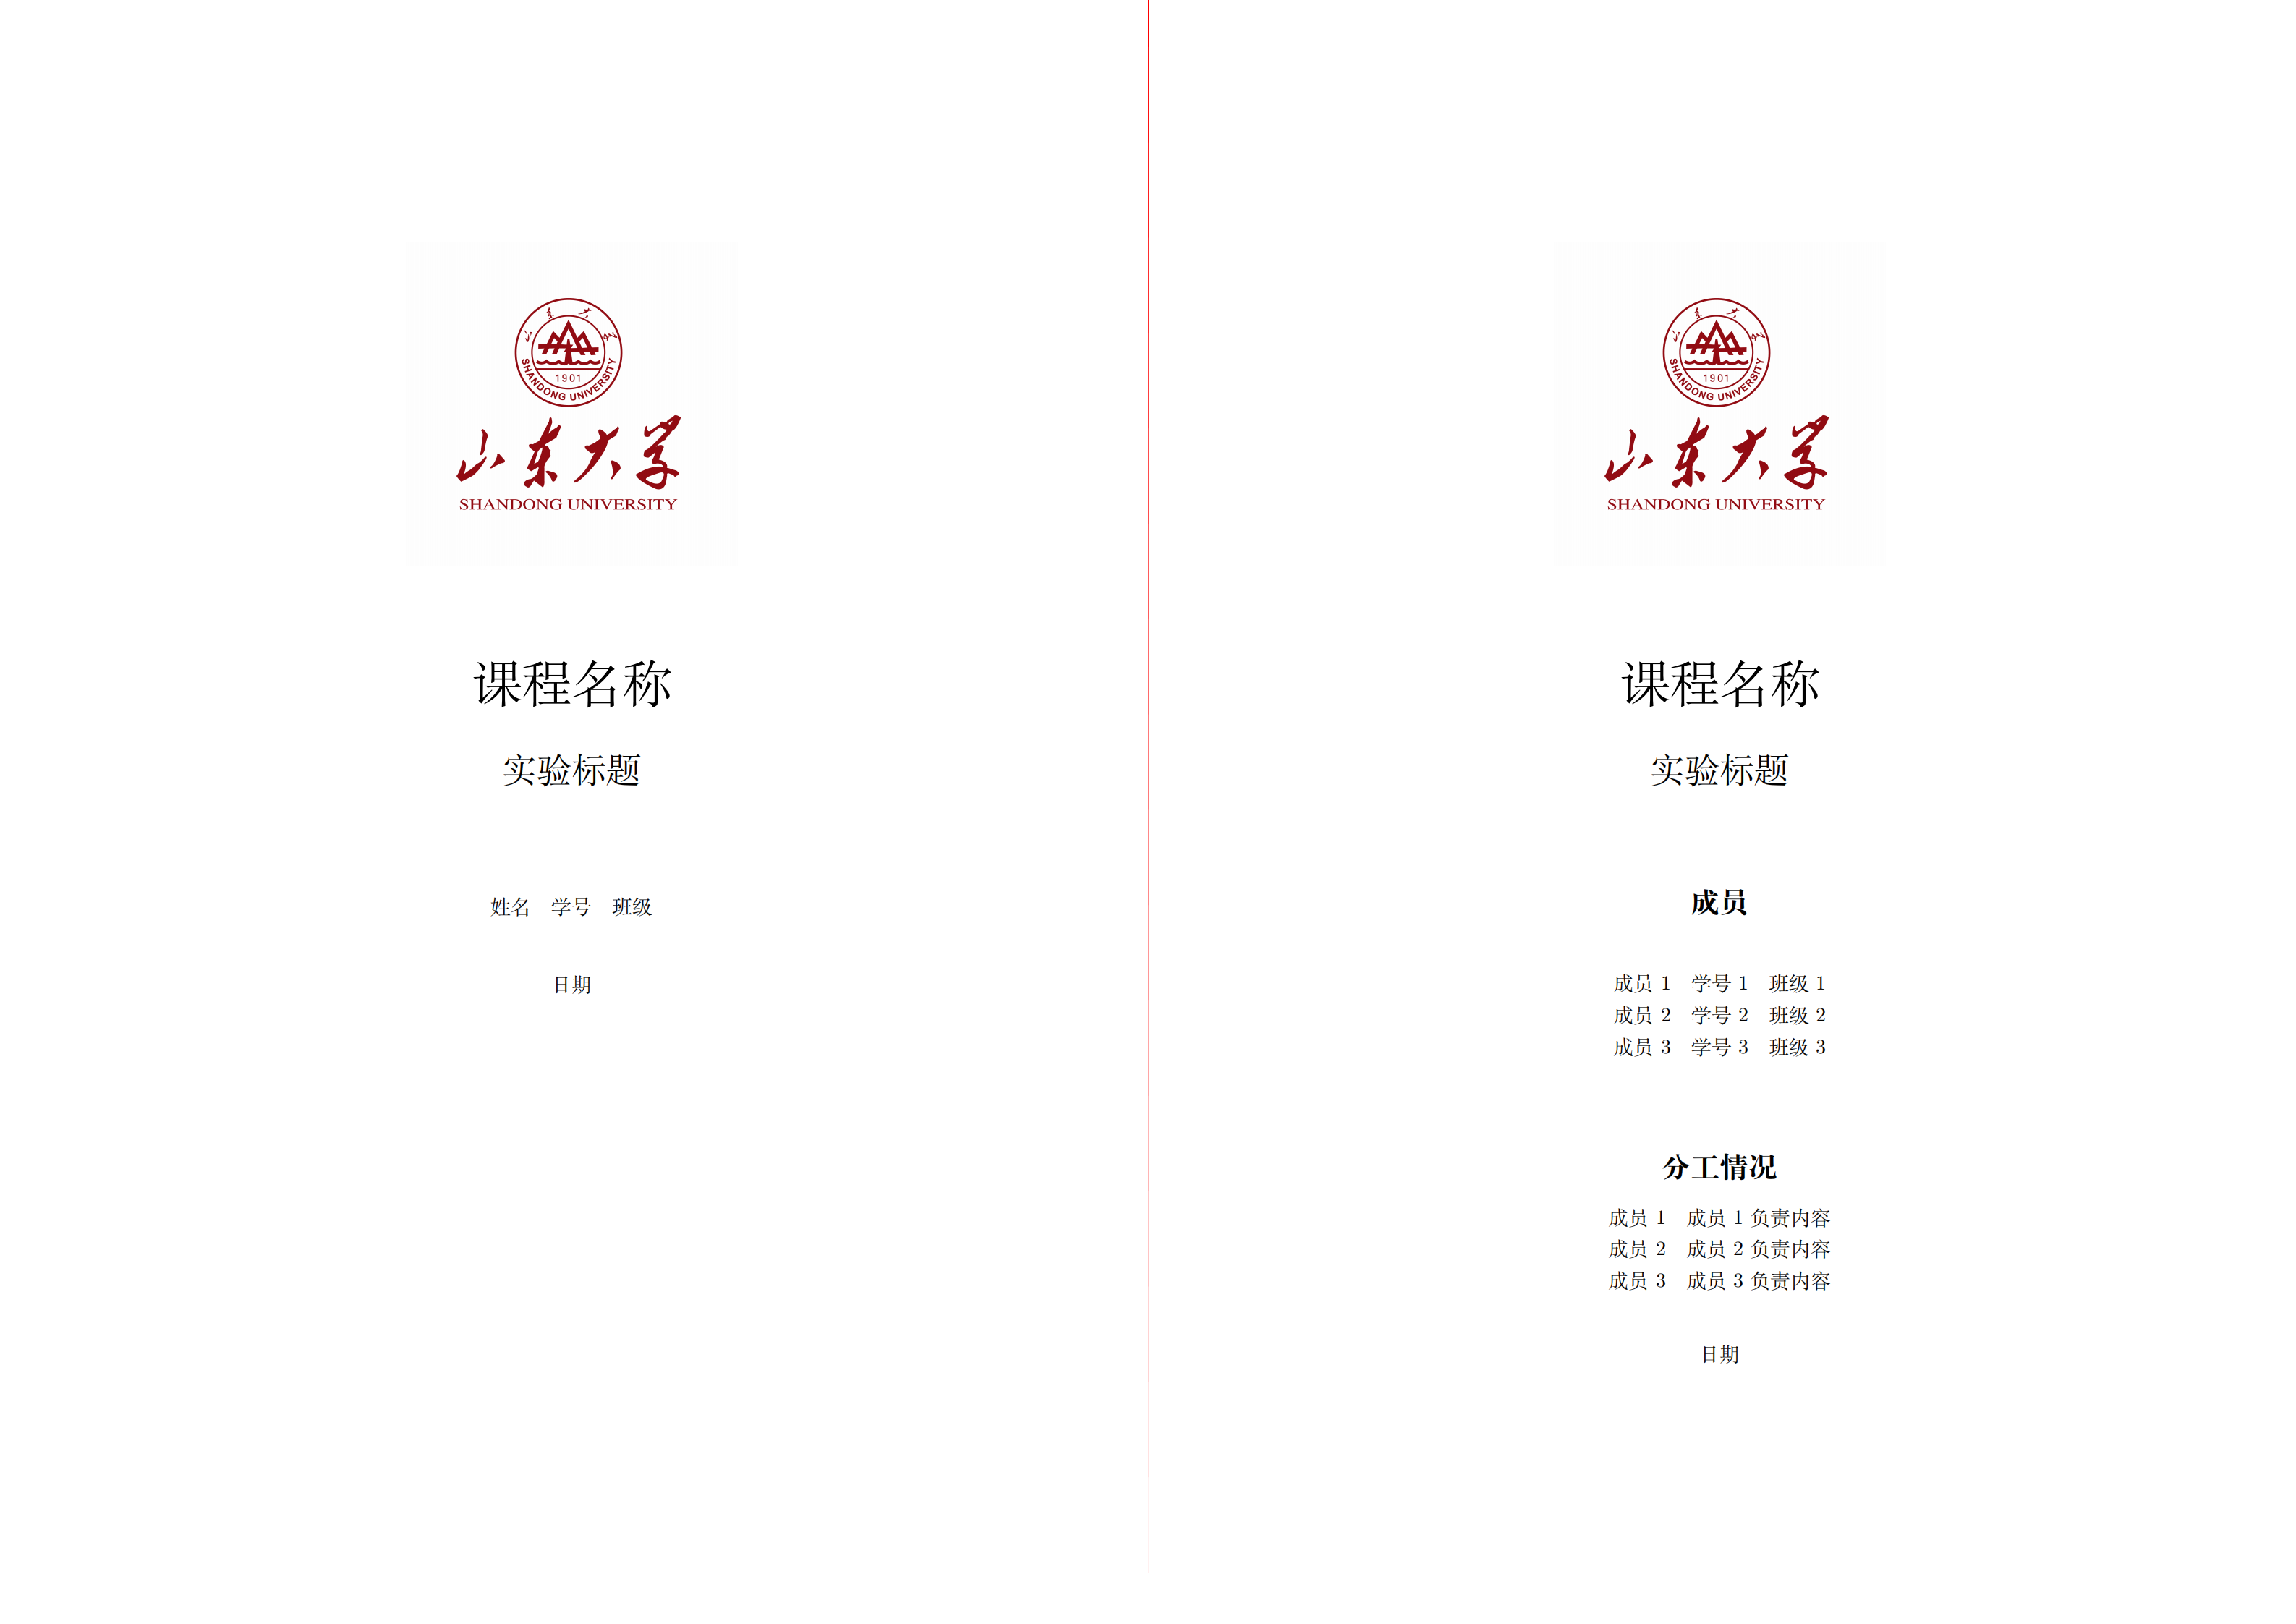
\includegraphics[width=\textwidth]{imgs/cover.png}
        \caption{两种封面样式}
        \label{fig:cover}
    \end{center}
\end{figure}

\section{个性化}

\subsection{字体}

本模板的中文默认字体为宋体,英文默认字体为 CM Roman,等宽默认字体为 Tex ecltt8。

使用 \mintinline{text}{fontspec} 宏包可以自定义字体。

使用 \mintinline{latex}{\setmainfont{fontname}} 命令可以设置正文字体(同时设置中文和英文),使用 \mintinline{latex}{\setmonofont{fontname}} 命令可以设置等宽字体,其中 \mintinline{latex}{fontname} 为字体名称。

使用 \mintinline{text}{fontspec} 宏包设置的字体应已安装在系统环境中,字体名称为字体家族名称,而非字体文件名。

\subsection{颜色}

使用 \mintinline{text}{xcolor} 宏包可以自定义颜色。

使用 \mintinline{latex}{\definecolor{colorname}{colortype}{colorvalue}} 命令定义颜色,其中 \mintinline{latex}{colorname} 为颜色名称,\mintinline{latex}{colortype} 为颜色类型,\mintinline{latex}{colorvalue} 为颜色值。常用的颜色类型有:\mintinline{text}{rgb}(RGB 颜色)、\mintinline{text}{cmyk}(CMYK 颜色)、\mintinline{latex}{bahs}(HTML 颜色)。

使用 \mintinline{latex}{\textcolor{color}{text}} 命令可以设置文本颜色,其中 \mintinline{latex}{color} 为颜色名称,\mintinline{latex}{text} 为文本内容。

下面以\cref{lst:22} 中的代码为例,展示自定义颜色的示例代码。

\begin{center}
    \captionof{listing}{自定义颜色示例代码}
    \label{lst:22}
    \begin{minted}{latex}
\definecolor{mycolor}{rgb}{12,125,200}
\textcolor{mycolor}{这段文字的颜色为自定义颜色。}
    \end{minted}
\end{center}

\cref{lst:22} 中的代码经过编译后,输出结果如下所示。

\vspace{0.75cm}
\hrule
\vspace{0.25cm}

\definecolor{mycolor}{RGB}{12,125,200}
\textcolor{mycolor}{这段文字的颜色为自定义颜色。}

\vspace{0.25cm}
\hrule
\vspace{0.25cm}

\subsection{页边距}

使用 \mintinline{text}{geometry} 宏包可以自定义页边距。

使用 \mintinline{latex}{\geometry{left=...,right=...,top=...,bottom=...}} 命令可以设置页边距,其中 \mintinline{latex}{left}、\mintinline{latex}{right}、\mintinline{latex}{top}、\mintinline{latex}{bottom} 可以分别设置上、下、左、右的页边距。

下面以\cref{lst:23} 中的代码为例,展示自定义页边距示例代码,本模板也设置为下面的样式。

\begin{center}
    \captionof{listing}{自定义页边距示例代码}
    \label{lst:23}
    \begin{minted}{latex}
\geometry{
    left=3.17cm,
    right=3.17cm,
    top=2.54cm,
    left=2.54cm
}
    \end{minted}
\end{center}

\subsection{代码高亮}

本模板使用 \mintinline{text}{minted} 宏包实现代码高亮。

\mintinline{text}{minted} 宏包依赖于Python的 \mintinline{text}{Pygments} 包实现代码高亮,而 \mintinline{text}{Pygments} 包支持数百种编程语言、模板语言与标记语言,因而大部分情况下无需担心语言不支持的问题。

使用 \mintinline{latex}{\usemintedstyle{style}} 命令可设置代码高亮风格,其中 \mintinline{latex}{style} 为风格名称。

使用 \mintinline{latex}{\setminted{options}} 命令可设置代码选项,其中 \mintinline{latex}{options} 为选项列表。常用选项有:\mintinline{latex}{linenos}(显示行号)、\mintinline{latex}{breaklines}(自动折行)、\mintinline{latex}{frame=single}(添加边框)、\mintinline{latex}{tabsize=4}(设置制表符宽度)、\mintinline{latex}{encoding=utf8}(设置编码)。

更多选项可以查看 \href{https://mirror.math.princeton.edu/pub/CTAN/macros/latex/contrib/minted/minted.pdf}{\mintinline{text}{minted} 宏包的官方文档}

下面以\cref{lst:24} 中的代码为例,展示 \mintinline{text}{minted} 宏包选项的设置方法,本模板也设置为下面的样式。

\begin{center}
    \captionof{listing}{\mintinline{text}{minted} 宏包选项示例代码}
    \label{lst:24}
    \begin{minted}{latex}
\setminted{
    linenos,
    breaklines,
	frame=single,
	tabsize=4,
	encoding=utf8,
}
    \end{minted}
\end{center}

\subsection{超链接}

使用 \mintinline{latex}{\hypersetup{...}} 命令可以对超链接样式做个性化设置。其中,\mintinline{latex}{...} 为设置项列表。常用设置项有:\mintinline{latex}{colorlinks}(设置链接颜色)、\mintinline{latex}{linkcolor}(设置内部链接颜色)、\mintinline{latex}{citecolor}(设置引用链接颜色)、\mintinline{latex}{urlcolor}(设置URL链接颜色)。更多设置项可以查看 \href{https://mirror.math.princeton.edu/pub/CTAN/macros/latex/contrib/hyperref/doc/hyperref-doc.pdf}{\mintinline{text}{hyperref} 宏包的官方文档}。

下面以\cref{lst:25} 中的代码为例,展示超链接样式设置的示例代码,本模板也设置为下面的样式。

\begin{center}
    \captionof{listing}{超链接样式设置示例代码}
    \label{lst:25}
    \begin{minted}{latex}
\hypersetup{
    hidelinks,
    colorlinks=true,
    linkcolor=blue,
    filecolor=blue,      
    urlcolor=blue,
    citecolor=cyan,
}
    \end{minted}
\end{center}

\section{宏包}

本模板使用了以下宏包。

\begin{center}
    \begin{tabular}{|m{0.45\textwidth}|m{0.45\textwidth}|}
        \hline
        宏包 & 说明 \\
        \hline
        \mintinline{text}{abstract} & 设置摘要 \\
        \mintinline{text}{amsmath} & 插入数学公式 \\
        \mintinline{text}{amsfonts} & 插入数学字体 \\
        \mintinline{text}{amssymb} & 插入数学符号 \\
        \mintinline{text}{authblk} & 处理作者信息 \\
        \mintinline{text}{booktabs} & 生成表格 \\
        \mintinline{text}{caption} & 图表标题设置 \\
        \mintinline{text}{cite} & 管理参考文献引用 \\
        \mintinline{text}{cleveref} & 重定义引用 \\
        \mintinline{text}{ctex} & 提供中文支持 \\
        \mintinline{text}{float} & 设置图片位置 \\
        \mintinline{text}{fontspec} & 设置字体 \\
        \mintinline{text}{graphicx} & 图片插入 \\
        \mintinline{text}{geometry} & 设置页边距 \\
        \mintinline{text}{hyperref} & 超链接 \\
        \mintinline{text}{minted} & 插入代码 \\
        \mintinline{text}{multicol} & 提供多栏排版支持 \\
        \mintinline{text}{sectsty} & 设置章节标题 \\
        \mintinline{text}{siunitx} & 插入单位 \\
        \mintinline{text}{subcaption} & 插入子图表标题 \\
        \mintinline{text}{tikz} & 绘制图表 \\
        \mintinline{text}{xcolor} & 设置自定义颜色 \\
        \hline
    \end{tabular}
\end{center}


\end{document}